\documentclass[10pt]{article}
\usepackage[a4paper, total={6in, 8in}]{geometry}


% ----------------------- Packages --------------------------

\usepackage[utf8]{inputenc}
\usepackage{babel}
%\decimalpoint


\usepackage{mathtools}% http://ctan.org/pkg/mathtool
\usepackage{amsthm, amsmath, bm, amssymb} %math packages
\usepackage{lineno} %Para enumerar las lineas



% -------------------------------------HIGHLIGHT-------

\usepackage[dvipsnames]{xcolor}
%\newcommand{\mathcolorbox}[2]{\colorbox{#1}{$\displaystyle #2$}}
\usepackage{color, soul}
\usepackage{hyperref}
\newcommand{\hlgray}[1]{{\sethlcolor{lightgray}\hl{#1}}}


% ----------------------------------------------FIGURAS-----------
\usepackage{tikz}
\tikzset{every picture/.style={line width=0.75pt}} %set default line width to 0.75pt 

\usepackage{subcaption, threeparttable}
\usepackage{graphicx} 

\usepackage{marginfix}
\usepackage{marginnote}
\renewcommand*{\marginfont}{\footnotesize} %Para cambiar el tamaño de fuente de las marginnote: https://tex.stackexchange.com/questions/30473/specifying-font-size-in-a-newcommand



%Paquetes usados en estilo.tex
\usepackage[font=footnotesize,format=plain,labelfont={bf,sf},textfont={it},width=10pt]{caption}
% Captions at the side of the page
%\usepackage[wide]{sidecap}
\usepackage{morefloats}
\usepackage{float}

\newcommand*{\IR}{\mathbb{R}}
\newcommand*{\IN}{\mathbb{N}}
\newcommand*{\IZ}{\mathbb{Z}}
\newcommand*{\IT}{\mathbb{T}}
\newcommand*{\QEDB}{\null\nobreak\hfill\ensuremath{\square}}%
\newcommand*{\diam}{\null\nobreak\hfill\ensuremath{\diamond}}%

\newcommand{\TODO}[1]{\textcolor{violet}{#1}} % TODO quitar. Sólo lo uso mientras estoy editando para resaltar en morado.


% -------------------------------------- AMBIENTES -----------------

\let\newemptytheorem\newtheorem
\usepackage{thmbox}

\newemptytheorem{ejemplo}{Ejemplo}


			\newtheorem[M]{teo}{Teorema}[section]
			%Pongo a todas el contador de 'teo'
			\newtheorem[M]{listaObj}[teo]{Lista de deseos}
			\newtheorem[M]{preg}[teo]{Pregunta}
			\newtheorem[M]{lema}[teo]{Lema}
			\newtheorem[M]{hip}[teo]{Hipótesis}
			\newtheorem[M]{prop}[teo]{Proposición}
			\newtheorem[M]{obs}[teo]{Observación}
			\newtheorem[M]{cor}[teo]{Corolario}
			\newtheorem[M]{defi}[teo]{Definición}
			\newtheorem[M]{notacion}[teo]{Notación}
			\newtheorem[M]{nota}[teo]{Nota}
			\newtheorem{pregunta}{Pregunta}

			


\usepackage{subfiles} % Best loaded last in the preamble
%%%%%%%%%%%%%%%%%%%%%%%%%%%%%%%%%%%%%%%%%%%%%%%%%%%%%%%%%%%%%%%%%%%%%%%%%%%%


\begin{document}
\begin{flushright}
\textbf{Amélie Bernès}
\end{flushright}

\section{Igualadores (Equalizers)}
En una categoría $\mathcal{A}$, un \textbf{igualador}
$(Z, h: Z \longrightarrow X)$ para dos morfismos 
$f, g : X \longrightarrow Y$ es una pareja tal que 

\begin{minipage}{0.5\textwidth}
\begin{itemize}
	\item $f \circ h = g \circ h$
	\item Si $W$ es otro objeto y $k : W \longrightarrow X$
	es tal que $f \circ k = g \circ k$, entonces
	existe un único morfismo $\phi: W \longrightarrow Z$
	tal que $k = h \circ \phi$. 
\end{itemize}
\end{minipage} \hfill
\begin{minipage}{0.45\textwidth}

\begin{center}
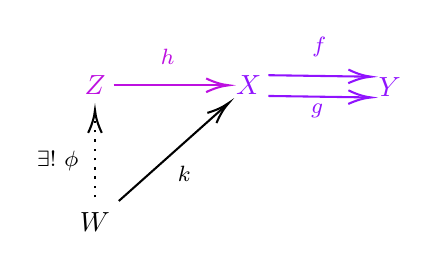
\begin{tikzpicture}[x=0.75pt,y=0.75pt,yscale=-1,xscale=1]
%uncomment if require: \path (0,235); %set diagram left start at 0, and has height of 235


% Text Node
\draw (194,91.57) node  [color={rgb, 255:red, 144; green, 19; blue, 254 }  ,opacity=1 ]  {$X$};
% Text Node
\draw (120,91.57) node  [color={rgb, 255:red, 189; green, 16; blue, 224 }  ,opacity=1 ]  {$Z$};
% Text Node
\draw (262,92.57) node  [color={rgb, 255:red, 144; green, 19; blue, 254 }  ,opacity=1 ]  {$Y$};
% Text Node
\draw (228,73) node  [font=\footnotesize,color={rgb, 255:red, 144; green, 19; blue, 254 }  ,opacity=1 ]  {$f$};
% Text Node
\draw (227,104) node  [font=\footnotesize,color={rgb, 255:red, 144; green, 19; blue, 254 }  ,opacity=1 ]  {$g$};
% Text Node
\draw (155,78) node  [font=\footnotesize,color={rgb, 255:red, 189; green, 16; blue, 224 }  ,opacity=1 ]  {$h$};
% Text Node
\draw (120,157.57) node    {$W$};
% Text Node
\draw (163,134) node  [font=\footnotesize,color={rgb, 255:red, 0; green, 0; blue, 0 }  ,opacity=1 ]  {$k$};
% Text Node
\draw (102,128) node  [font=\footnotesize,color={rgb, 255:red, 0; green, 0; blue, 0 }  ,opacity=1 ]  {$\exists !\ \phi $};
% Connection
\draw [color={rgb, 255:red, 189; green, 16; blue, 224 }  ,draw opacity=1 ]   (129,91.57) -- (182.5,91.57) ;
\draw [shift={(184.5,91.57)}, rotate = 180] [color={rgb, 255:red, 189; green, 16; blue, 224 }  ,draw opacity=1 ][line width=0.75]    (10.93,-3.29) .. controls (6.95,-1.4) and (3.31,-0.3) .. (0,0) .. controls (3.31,0.3) and (6.95,1.4) .. (10.93,3.29)   ;
% Connection
\draw [color={rgb, 255:red, 144; green, 19; blue, 254 }  ,draw opacity=1 ]   (203.5,86.71) -- (251,87.41) ;
\draw [shift={(253,87.44)}, rotate = 180.84] [color={rgb, 255:red, 144; green, 19; blue, 254 }  ,draw opacity=1 ][line width=0.75]    (10.93,-3.29) .. controls (6.95,-1.4) and (3.31,-0.3) .. (0,0) .. controls (3.31,0.3) and (6.95,1.4) .. (10.93,3.29)   ;
% Connection
\draw [color={rgb, 255:red, 144; green, 19; blue, 254 }  ,draw opacity=1 ]   (203.5,96.71) -- (251,97.41) ;
\draw [shift={(253,97.44)}, rotate = 180.84] [color={rgb, 255:red, 144; green, 19; blue, 254 }  ,draw opacity=1 ][line width=0.75]    (10.93,-3.29) .. controls (6.95,-1.4) and (3.31,-0.3) .. (0,0) .. controls (3.31,0.3) and (6.95,1.4) .. (10.93,3.29)   ;
% Connection
\draw    (131.5,147.31) -- (183.01,101.38) ;
\draw [shift={(184.5,100.04)}, rotate = 138.27] [color={rgb, 255:red, 0; green, 0; blue, 0 }  ][line width=0.75]    (10.93,-3.29) .. controls (6.95,-1.4) and (3.31,-0.3) .. (0,0) .. controls (3.31,0.3) and (6.95,1.4) .. (10.93,3.29)   ;
% Connection
\draw  [dash pattern={on 0.84pt off 2.51pt}]  (120,145.57) -- (120,105.57) ;
\draw [shift={(120,103.57)}, rotate = 90] [color={rgb, 255:red, 0; green, 0; blue, 0 }  ][line width=0.75]    (10.93,-3.29) .. controls (6.95,-1.4) and (3.31,-0.3) .. (0,0) .. controls (3.31,0.3) and (6.95,1.4) .. (10.93,3.29)   ;
\end{tikzpicture}

\end{center}
\end{minipage}

\begin{prop}
Si $h: Z \longrightarrow X$ es el igualador de un par de morfismos,
entonces $h$ es un monomorfismo (i.e. cancelable por la izquierda).
\end{prop}
\noindent
\textbf{Demostración.}
En efecto, sean $p, q: A \longrightarrow Z$ morfismos tales que 
$h \circ q = h \circ p$.
Entonces, como $f \circ h = g \circ h$, también
\[
f \circ (h \circ p) = (f \circ h) \circ p 
= (g \circ h) \circ p = g \circ (h \circ p).
\]
Luego, existe un único $\phi : A \longrightarrow Z$ tal que 
\[
h \circ \phi = h \circ p.
\]
Tanto $\phi = p$ como $\phi = q$ funcionan, luego, $p = q$.

\begin{center}
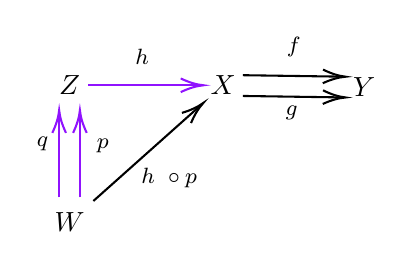
\begin{tikzpicture}[x=0.75pt,y=0.75pt,yscale=-1,xscale=1]
%uncomment if require: \path (0,235); %set diagram left start at 0, and has height of 235


% Text Node
\draw (194,91.57) node  [color={rgb, 255:red, 0; green, 0; blue, 0 }  ,opacity=1 ]  {$X$};
% Text Node
\draw (120,91.57) node  [color={rgb, 255:red, 0; green, 0; blue, 0 }  ,opacity=1 ]  {$Z$};
% Text Node
\draw (262,92.57) node  [color={rgb, 255:red, 0; green, 0; blue, 0 }  ,opacity=1 ]  {$Y$};
% Text Node
\draw (228,73) node  [font=\footnotesize,color={rgb, 255:red, 0; green, 0; blue, 0 }  ,opacity=1 ]  {$f$};
% Text Node
\draw (227,105) node  [font=\footnotesize,color={rgb, 255:red, 0; green, 0; blue, 0 }  ,opacity=1 ]  {$g$};
% Text Node
\draw (155,78) node  [font=\footnotesize,color={rgb, 255:red, 0; green, 0; blue, 0 }  ,opacity=1 ]  {$h$};
% Text Node
\draw (120,157.57) node    {$W$};
% Text Node
\draw (168,136) node  [font=\footnotesize,color={rgb, 255:red, 0; green, 0; blue, 0 }  ,opacity=1 ]  {$h\ \circ p$};
% Text Node
\draw (107,120) node  [font=\footnotesize,color={rgb, 255:red, 0; green, 0; blue, 0 }  ,opacity=1 ]  {$q$};
% Text Node
\draw (136,121) node  [font=\footnotesize,color={rgb, 255:red, 0; green, 0; blue, 0 }  ,opacity=1 ]  {$p$};
% Connection
\draw [color={rgb, 255:red, 144; green, 19; blue, 254 }  ,draw opacity=1 ]   (129,91.57) -- (182.5,91.57) ;
\draw [shift={(184.5,91.57)}, rotate = 180] [color={rgb, 255:red, 144; green, 19; blue, 254 }  ,draw opacity=1 ][line width=0.75]    (10.93,-3.29) .. controls (6.95,-1.4) and (3.31,-0.3) .. (0,0) .. controls (3.31,0.3) and (6.95,1.4) .. (10.93,3.29)   ;
% Connection
\draw [color={rgb, 255:red, 0; green, 0; blue, 0 }  ,draw opacity=1 ]   (203.5,86.71) -- (251,87.41) ;
\draw [shift={(253,87.44)}, rotate = 180.84] [color={rgb, 255:red, 0; green, 0; blue, 0 }  ,draw opacity=1 ][line width=0.75]    (10.93,-3.29) .. controls (6.95,-1.4) and (3.31,-0.3) .. (0,0) .. controls (3.31,0.3) and (6.95,1.4) .. (10.93,3.29)   ;
% Connection
\draw [color={rgb, 255:red, 0; green, 0; blue, 0 }  ,draw opacity=1 ]   (203.5,96.71) -- (251,97.41) ;
\draw [shift={(253,97.44)}, rotate = 180.84] [color={rgb, 255:red, 0; green, 0; blue, 0 }  ,draw opacity=1 ][line width=0.75]    (10.93,-3.29) .. controls (6.95,-1.4) and (3.31,-0.3) .. (0,0) .. controls (3.31,0.3) and (6.95,1.4) .. (10.93,3.29)   ;
% Connection
\draw [color={rgb, 255:red, 0; green, 0; blue, 0 }  ,draw opacity=1 ]   (131.5,147.31) -- (183.01,101.38) ;
\draw [shift={(184.5,100.04)}, rotate = 138.27] [color={rgb, 255:red, 0; green, 0; blue, 0 }  ,draw opacity=1 ][line width=0.75]    (10.93,-3.29) .. controls (6.95,-1.4) and (3.31,-0.3) .. (0,0) .. controls (3.31,0.3) and (6.95,1.4) .. (10.93,3.29)   ;
% Connection
\draw [color={rgb, 255:red, 144; green, 19; blue, 254 }  ,draw opacity=1 ]   (115,145.57) -- (115,105.57) ;
\draw [shift={(115,103.57)}, rotate = 90] [color={rgb, 255:red, 144; green, 19; blue, 254 }  ,draw opacity=1 ][line width=0.75]    (10.93,-3.29) .. controls (6.95,-1.4) and (3.31,-0.3) .. (0,0) .. controls (3.31,0.3) and (6.95,1.4) .. (10.93,3.29)   ;
% Connection
\draw [color={rgb, 255:red, 144; green, 19; blue, 254 }  ,draw opacity=1 ]   (125,145.57) -- (125,105.57) ;
\draw [shift={(125,103.57)}, rotate = 90] [color={rgb, 255:red, 144; green, 19; blue, 254 }  ,draw opacity=1 ][line width=0.75]    (10.93,-3.29) .. controls (6.95,-1.4) and (3.31,-0.3) .. (0,0) .. controls (3.31,0.3) and (6.95,1.4) .. (10.93,3.29)   ;

\end{tikzpicture}
\end{center}

\QEDB
\vspace{0.2cm}

\section{Categorías reflexivas, Nakagawa (Categorical Topology)}

Estamos suponiendo que en la categoría $\mathcal{A}$ existen todos los 
límites pequeños (p.ej. productos, igualadores) y que $\mathcal{B}$
es cerrada bajo isomorfismos.

\begin{lema}
\textbf{(Lema 7.10, Nakagawa)} Si $\mathcal{B}$ es fuertemente cerrada en 
$\mathcal{A}$ bajo igualadores, entonces $\mathcal{B}$ es cerrada en 
$\mathcal{A}$ bajo intersecciones de monomorfismos regulares.

\end{lema}
\textbf{Demostración.}
Sea $(h_{i}: Z \longrightarrow X)_{i \in I}$ una familia de monomorfismos
regulares con $X \in Obj(\mathcal{B})$; queremos demostrar que su intersección
está en $\mathcal{B}$. Para cada $i \in I$, sean 
$f_{i}, g_{i}: X \longrightarrow Y_{i}$ tales que 

       
\begin{center}
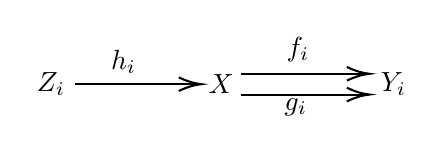
\begin{tikzpicture}[x=0.75pt,y=0.75pt,yscale=-1,xscale=1]
% Text Node
\draw (110,102.14) node    {$Z_{i}$};
% Text Node
\draw (192,102.14) node    {$X$};
% Text Node
\draw (145,91.29) node    {$h_{i}$};
% Text Node
\draw (275,102.14) node    {$Y_{i}$};
% Text Node
\draw (229,85.29) node    {$f_{i}$};
% Text Node
\draw (228,113.29) node    {$g_{i}$};
% Connection
\draw    (121.5,102.14) -- (180.5,102.14) ;
\draw [shift={(182.5,102.14)}, rotate = 180] [color={rgb, 255:red, 0; green, 0; blue, 0 }  ][line width=0.75]    (10.93,-3.29) .. controls (6.95,-1.4) and (3.31,-0.3) .. (0,0) .. controls (3.31,0.3) and (6.95,1.4) .. (10.93,3.29)   ;
% Connection
\draw    (201.5,97.14) -- (261.5,97.14) ;
\draw [shift={(263.5,97.14)}, rotate = 180] [color={rgb, 255:red, 0; green, 0; blue, 0 }  ][line width=0.75]    (10.93,-3.29) .. controls (6.95,-1.4) and (3.31,-0.3) .. (0,0) .. controls (3.31,0.3) and (6.95,1.4) .. (10.93,3.29)   ;
% Connection
\draw    (201.5,107.14) -- (261.5,107.14) ;
\draw [shift={(263.5,107.14)}, rotate = 180] [color={rgb, 255:red, 0; green, 0; blue, 0 }  ][line width=0.75]    (10.93,-3.29) .. controls (6.95,-1.4) and (3.31,-0.3) .. (0,0) .. controls (3.31,0.3) and (6.95,1.4) .. (10.93,3.29)   ;

\end{tikzpicture}
\end{center}
es un diagrama igualador. Entonces
\begin{equation}
	\label{eq: diagrama igualador i origin}
	\forall i \in I : \hspace{0.2cm} f_{i} \circ h_{i} = g_{i} \circ h_{i}.
\end{equation}
Sea $Y = \Pi_{i \in I} Y_{i}$, $p_{i}: Y \longrightarrow Y_{i}$
el producto de la familia $(Y_{i})_{i \in I}$
de objetos de 
$\mathcal{A}$ - que existe por ser la categoría $\mathcal{A}$ completa.
Sean $f, g: X \longrightarrow Y$ los únicos morfismos tales que 
\begin{equation}
	\label{eq: pi f y gi}
	\forall i \in I: \hspace{0.2cm} p_{i} \circ f = f_{i},
	\hspace{0.1cm}
	p_{i} \circ g = g_{i}.
\end{equation}

Por ser $\mathcal{A}$ completa, existe un monomorfismo igualador
$h: W \longrightarrow X$ para $f$ y $g$; 

\begin{equation}
	\label{eq: fh = gh}
	f \circ h = g \circ h. 
\end{equation}

Por ser $\mathcal{B}$ fuertemente
cerrada en $\mathcal{A}$ bajo igualadores y como 
$X \in Obj(\mathcal{B})$, entonces $W \in Obj(\mathcal{B})$.

\begin{center}
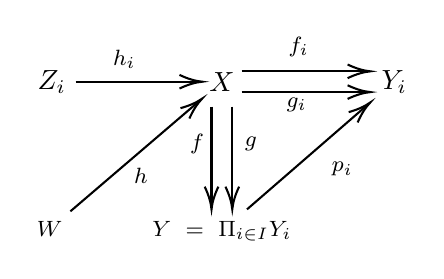
\begin{tikzpicture}[x=0.75pt,y=0.75pt,yscale=-1,xscale=1]
%uncomment if require: \path (0,235); %set diagram left start at 0, and has height of 235


% Text Node
\draw (110,102.14) node    {$Z_{i}$};
% Text Node
\draw (192,102.14) node    {$X$};
% Text Node
\draw (145,91.29) node  [font=\footnotesize]  {$h_{i}$};
% Text Node
\draw (275,102.14) node    {$Y_{i}$};
% Text Node
\draw (229,85.29) node  [font=\footnotesize]  {$f_{i}$};
% Text Node
\draw (228,113.29) node  [font=\footnotesize]  {$g_{i}$};
% Text Node
\draw (192,174.14) node  [font=\footnotesize]  {$Y\ =\ \Pi _{i\in I} Y_{i}$};
% Text Node
\draw (250,144.29) node  [font=\footnotesize]  {$p_{i}$};
% Text Node
\draw (180,132.29) node  [font=\footnotesize]  {$f$};
% Text Node
\draw (206,132.29) node  [font=\footnotesize]  {$g$};
% Text Node
\draw (109,173.14) node  [font=\footnotesize]  {$W$};
% Text Node
\draw (153,147.29) node  [font=\footnotesize]  {$h$};
% Connection
\draw    (121.5,102.14) -- (180.5,102.14) ;
\draw [shift={(182.5,102.14)}, rotate = 180] [color={rgb, 255:red, 0; green, 0; blue, 0 }  ][line width=0.75]    (10.93,-3.29) .. controls (6.95,-1.4) and (3.31,-0.3) .. (0,0) .. controls (3.31,0.3) and (6.95,1.4) .. (10.93,3.29)   ;
% Connection
\draw    (201.5,97.14) -- (261.5,97.14) ;
\draw [shift={(263.5,97.14)}, rotate = 180] [color={rgb, 255:red, 0; green, 0; blue, 0 }  ][line width=0.75]    (10.93,-3.29) .. controls (6.95,-1.4) and (3.31,-0.3) .. (0,0) .. controls (3.31,0.3) and (6.95,1.4) .. (10.93,3.29)   ;
% Connection
\draw    (201.5,107.14) -- (261.5,107.14) ;
\draw [shift={(263.5,107.14)}, rotate = 180] [color={rgb, 255:red, 0; green, 0; blue, 0 }  ][line width=0.75]    (10.93,-3.29) .. controls (6.95,-1.4) and (3.31,-0.3) .. (0,0) .. controls (3.31,0.3) and (6.95,1.4) .. (10.93,3.29)   ;
% Connection
\draw    (204.1,163.64) -- (261.99,113.43) ;
\draw [shift={(263.5,112.12)}, rotate = 139.06] [color={rgb, 255:red, 0; green, 0; blue, 0 }  ][line width=0.75]    (10.93,-3.29) .. controls (6.95,-1.4) and (3.31,-0.3) .. (0,0) .. controls (3.31,0.3) and (6.95,1.4) .. (10.93,3.29)   ;
% Connection
\draw    (197,114.14) -- (197,161.64) ;
\draw [shift={(197,163.64)}, rotate = 270] [color={rgb, 255:red, 0; green, 0; blue, 0 }  ][line width=0.75]    (10.93,-3.29) .. controls (6.95,-1.4) and (3.31,-0.3) .. (0,0) .. controls (3.31,0.3) and (6.95,1.4) .. (10.93,3.29)   ;
% Connection
\draw    (187,114.14) -- (187,161.64) ;
\draw [shift={(187,163.64)}, rotate = 270] [color={rgb, 255:red, 0; green, 0; blue, 0 }  ][line width=0.75]    (10.93,-3.29) .. controls (6.95,-1.4) and (3.31,-0.3) .. (0,0) .. controls (3.31,0.3) and (6.95,1.4) .. (10.93,3.29)   ;
% Connection
\draw    (119,164.59) -- (180.98,111.57) ;
\draw [shift={(182.5,110.27)}, rotate = 139.46] [color={rgb, 255:red, 0; green, 0; blue, 0 }  ][line width=0.75]    (10.93,-3.29) .. controls (6.95,-1.4) and (3.31,-0.3) .. (0,0) .. controls (3.31,0.3) and (6.95,1.4) .. (10.93,3.29)   ;

\end{tikzpicture}
\end{center}

Si $i \in I$, entonces, de \eqref{eq: pi f y gi} 
y \eqref{eq: fh = gh} se sigue que
\[
f_{i} \circ h = (p_{i} \circ f) \circ h = (p_{i} \circ g) \circ h
= g_{i} \circ h,
\]
luego, por ser $(Z_{i}, h_{i})$ igualador de $f_{i}, g_{i}$, se tiene que
existe $\omega_{i} : W \longrightarrow Z_{i}$ tal que 
\begin{equation}
	\label{eq: h = hi wi}
	h = h_{i} \circ \omega_{i}, \hspace{0.2cm} i \in I.
\end{equation}
\begin{center}
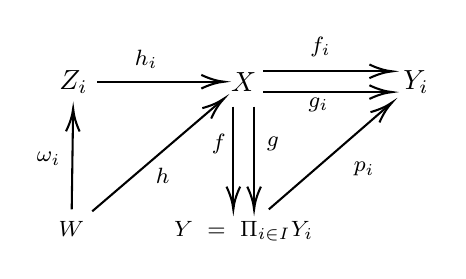
\begin{tikzpicture}[x=0.75pt,y=0.75pt,yscale=-1,xscale=1]
%uncomment if require: \path (0,235); %set diagram left start at 0, and has height of 235


% Text Node
\draw (110,102.14) node    {$Z_{i}$};
% Text Node
\draw (192,102.14) node    {$X$};
% Text Node
\draw (145,91.29) node  [font=\footnotesize]  {$h_{i}$};
% Text Node
\draw (275,102.14) node    {$Y_{i}$};
% Text Node
\draw (229,85.29) node  [font=\footnotesize]  {$f_{i}$};
% Text Node
\draw (228,113.29) node  [font=\footnotesize]  {$g_{i}$};
% Text Node
\draw (192,174.14) node  [font=\footnotesize]  {$Y\ =\ \Pi _{i\in I} Y_{i}$};
% Text Node
\draw (250,144.29) node  [font=\footnotesize]  {$p_{i}$};
% Text Node
\draw (180,132.29) node  [font=\footnotesize]  {$f$};
% Text Node
\draw (206,132.29) node  [font=\footnotesize]  {$g$};
% Text Node
\draw (109,173.14) node  [font=\footnotesize]  {$W$};
% Text Node
\draw (153,147.29) node  [font=\footnotesize]  {$h$};
% Text Node
\draw (98,139.29) node  [font=\footnotesize]  {$\omega _{i}$};
% Connection
\draw    (121.5,102.14) -- (180.5,102.14) ;
\draw [shift={(182.5,102.14)}, rotate = 180] [color={rgb, 255:red, 0; green, 0; blue, 0 }  ][line width=0.75]    (10.93,-3.29) .. controls (6.95,-1.4) and (3.31,-0.3) .. (0,0) .. controls (3.31,0.3) and (6.95,1.4) .. (10.93,3.29)   ;
% Connection
\draw    (201.5,97.14) -- (261.5,97.14) ;
\draw [shift={(263.5,97.14)}, rotate = 180] [color={rgb, 255:red, 0; green, 0; blue, 0 }  ][line width=0.75]    (10.93,-3.29) .. controls (6.95,-1.4) and (3.31,-0.3) .. (0,0) .. controls (3.31,0.3) and (6.95,1.4) .. (10.93,3.29)   ;
% Connection
\draw    (201.5,107.14) -- (261.5,107.14) ;
\draw [shift={(263.5,107.14)}, rotate = 180] [color={rgb, 255:red, 0; green, 0; blue, 0 }  ][line width=0.75]    (10.93,-3.29) .. controls (6.95,-1.4) and (3.31,-0.3) .. (0,0) .. controls (3.31,0.3) and (6.95,1.4) .. (10.93,3.29)   ;
% Connection
\draw    (204.1,163.64) -- (261.99,113.43) ;
\draw [shift={(263.5,112.12)}, rotate = 139.06] [color={rgb, 255:red, 0; green, 0; blue, 0 }  ][line width=0.75]    (10.93,-3.29) .. controls (6.95,-1.4) and (3.31,-0.3) .. (0,0) .. controls (3.31,0.3) and (6.95,1.4) .. (10.93,3.29)   ;
% Connection
\draw    (197,114.14) -- (197,161.64) ;
\draw [shift={(197,163.64)}, rotate = 270] [color={rgb, 255:red, 0; green, 0; blue, 0 }  ][line width=0.75]    (10.93,-3.29) .. controls (6.95,-1.4) and (3.31,-0.3) .. (0,0) .. controls (3.31,0.3) and (6.95,1.4) .. (10.93,3.29)   ;
% Connection
\draw    (187,114.14) -- (187,161.64) ;
\draw [shift={(187,163.64)}, rotate = 270] [color={rgb, 255:red, 0; green, 0; blue, 0 }  ][line width=0.75]    (10.93,-3.29) .. controls (6.95,-1.4) and (3.31,-0.3) .. (0,0) .. controls (3.31,0.3) and (6.95,1.4) .. (10.93,3.29)   ;
% Connection
\draw    (119,164.59) -- (180.98,111.57) ;
\draw [shift={(182.5,110.27)}, rotate = 139.46] [color={rgb, 255:red, 0; green, 0; blue, 0 }  ][line width=0.75]    (10.93,-3.29) .. controls (6.95,-1.4) and (3.31,-0.3) .. (0,0) .. controls (3.31,0.3) and (6.95,1.4) .. (10.93,3.29)   ;
% Connection
\draw    (109.13,163.64) -- (109.79,117.14) ;
\draw [shift={(109.82,115.14)}, rotate = 90.81] [color={rgb, 255:red, 0; green, 0; blue, 0 }  ][line width=0.75]    (10.93,-3.29) .. controls (6.95,-1.4) and (3.31,-0.3) .. (0,0) .. controls (3.31,0.3) and (6.95,1.4) .. (10.93,3.29)   ;

\end{tikzpicture}
\end{center}
Si mostramos que $[W, ( (\omega)_{i \in I}, h ) ]$ es una intersección 
de la familia de monomorfismos regulares $(h_{i})_{i \in I}$, puesto que ya
vimos que $W \in Obj(\mathcal{B})$, habremos acabado.

Sean pues para $i \in I$,
$\omega_{i}' : U \longrightarrow Z_{i}$ y
$h' : U \longrightarrow X$ monomorfismos tales que
\begin{equation}
	\label{eq: hi omega i prima = h prima}
\forall i \in I: \hspace{0.2cm} h_{i} \circ \omega_{i}' = h'.
\end{equation}

\begin{center}
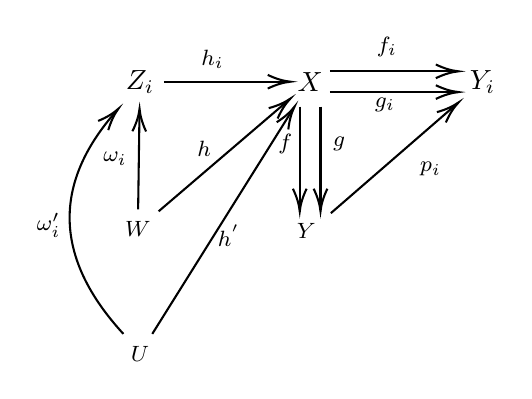
\begin{tikzpicture}[x=0.75pt,y=0.75pt,yscale=-1,xscale=1]
%uncomment if require: \path (0,235); %set diagram left start at 0, and has height of 235


% Text Node
\draw (169,66.14) node    {$Z_{i}$};
% Text Node
\draw (251,66.14) node    {$X$};
% Text Node
\draw (204,55.29) node  [font=\footnotesize]  {$h_{i}$};
% Text Node
\draw (334,66.14) node    {$Y_{i}$};
% Text Node
\draw (288,49.29) node  [font=\footnotesize]  {$f_{i}$};
% Text Node
\draw (287,77.29) node  [font=\footnotesize]  {$g_{i}$};
% Text Node
\draw (251,138.14) node  [font=\footnotesize]  {$Y\ $};
% Text Node
\draw (309,108.29) node  [font=\footnotesize]  {$p_{i}$};
% Text Node
\draw (239,96.29) node  [font=\footnotesize]  {$f$};
% Text Node
\draw (265,96.29) node  [font=\footnotesize]  {$g$};
% Text Node
\draw (168,137.14) node  [font=\footnotesize]  {$W$};
% Text Node
\draw (200,98.29) node  [font=\footnotesize]  {$h$};
% Text Node
\draw (157,103.29) node  [font=\footnotesize]  {$\omega _{i}$};
% Text Node
\draw (169,197.14) node  [font=\footnotesize]  {$U$};
% Text Node
\draw (212,140.29) node  [font=\footnotesize]  {$h^{'}$};
% Text Node
\draw (125,135.29) node  [font=\footnotesize]  {$\omega _{i} '$};
% Connection
\draw    (180.5,66.14) -- (239.5,66.14) ;
\draw [shift={(241.5,66.14)}, rotate = 180] [color={rgb, 255:red, 0; green, 0; blue, 0 }  ][line width=0.75]    (10.93,-3.29) .. controls (6.95,-1.4) and (3.31,-0.3) .. (0,0) .. controls (3.31,0.3) and (6.95,1.4) .. (10.93,3.29)   ;
% Connection
\draw    (260.5,61.14) -- (320.5,61.14) ;
\draw [shift={(322.5,61.14)}, rotate = 180] [color={rgb, 255:red, 0; green, 0; blue, 0 }  ][line width=0.75]    (10.93,-3.29) .. controls (6.95,-1.4) and (3.31,-0.3) .. (0,0) .. controls (3.31,0.3) and (6.95,1.4) .. (10.93,3.29)   ;
% Connection
\draw    (260.5,71.14) -- (320.5,71.14) ;
\draw [shift={(322.5,71.14)}, rotate = 180] [color={rgb, 255:red, 0; green, 0; blue, 0 }  ][line width=0.75]    (10.93,-3.29) .. controls (6.95,-1.4) and (3.31,-0.3) .. (0,0) .. controls (3.31,0.3) and (6.95,1.4) .. (10.93,3.29)   ;
% Connection
\draw    (261,129.47) -- (320.99,77.43) ;
\draw [shift={(322.5,76.12)}, rotate = 139.06] [color={rgb, 255:red, 0; green, 0; blue, 0 }  ][line width=0.75]    (10.93,-3.29) .. controls (6.95,-1.4) and (3.31,-0.3) .. (0,0) .. controls (3.31,0.3) and (6.95,1.4) .. (10.93,3.29)   ;
% Connection
\draw    (256,78.14) -- (256,126.64) ;
\draw [shift={(256,128.64)}, rotate = 270] [color={rgb, 255:red, 0; green, 0; blue, 0 }  ][line width=0.75]    (10.93,-3.29) .. controls (6.95,-1.4) and (3.31,-0.3) .. (0,0) .. controls (3.31,0.3) and (6.95,1.4) .. (10.93,3.29)   ;
% Connection
\draw    (246,78.14) -- (246,126.64) ;
\draw [shift={(246,128.64)}, rotate = 270] [color={rgb, 255:red, 0; green, 0; blue, 0 }  ][line width=0.75]    (10.93,-3.29) .. controls (6.95,-1.4) and (3.31,-0.3) .. (0,0) .. controls (3.31,0.3) and (6.95,1.4) .. (10.93,3.29)   ;
% Connection
\draw    (178,128.59) -- (239.98,75.57) ;
\draw [shift={(241.5,74.27)}, rotate = 139.46] [color={rgb, 255:red, 0; green, 0; blue, 0 }  ][line width=0.75]    (10.93,-3.29) .. controls (6.95,-1.4) and (3.31,-0.3) .. (0,0) .. controls (3.31,0.3) and (6.95,1.4) .. (10.93,3.29)   ;
% Connection
\draw    (168.13,127.64) -- (168.79,81.14) ;
\draw [shift={(168.82,79.14)}, rotate = 90.81] [color={rgb, 255:red, 0; green, 0; blue, 0 }  ][line width=0.75]    (10.93,-3.29) .. controls (6.95,-1.4) and (3.31,-0.3) .. (0,0) .. controls (3.31,0.3) and (6.95,1.4) .. (10.93,3.29)   ;
% Connection
\draw    (174.95,187.64) -- (242.43,79.84) ;
\draw [shift={(243.49,78.14)}, rotate = 122.04] [color={rgb, 255:red, 0; green, 0; blue, 0 }  ][line width=0.75]    (10.93,-3.29) .. controls (6.95,-1.4) and (3.31,-0.3) .. (0,0) .. controls (3.31,0.3) and (6.95,1.4) .. (10.93,3.29)   ;
% Connection
\draw    (161.03,187.64) .. controls (127.64,151.27) and (126.52,115.45) .. (157.69,80.21) ;
\draw [shift={(158.64,79.14)}, rotate = 132.09] [color={rgb, 255:red, 0; green, 0; blue, 0 }  ][line width=0.75]    (10.93,-3.29) .. controls (6.95,-1.4) and (3.31,-0.3) .. (0,0) .. controls (3.31,0.3) and (6.95,1.4) .. (10.93,3.29)   ;

\end{tikzpicture}

\end{center}

Entonces, para toda $i \in I$,
por \eqref{eq: diagrama igualador i origin},
\begin{equation}
	\label{eq: fi circ h' igual gi circ h'}
f_{i} \circ h' = (f_{i} \circ h_{i}) \circ \omega_{i}' 
= (g_{i} \circ h_{i}) \circ \omega_{i}' = g_{i} \circ h',
\end{equation}
por lo tanto,
\begin{equation}
	\label{eq: f circ h' g circ h'}
	f \circ h' = g \circ h'. 
\end{equation}
Como $(W, h)$ es un igualador para $f$ y $g$, existe un único
morfismo $\phi : U \longrightarrow W$ tal que 
\begin{equation}
	\label{ eq: h' igual h circ phi}
	h' = h \circ \phi
\end{equation}
\begin{center}
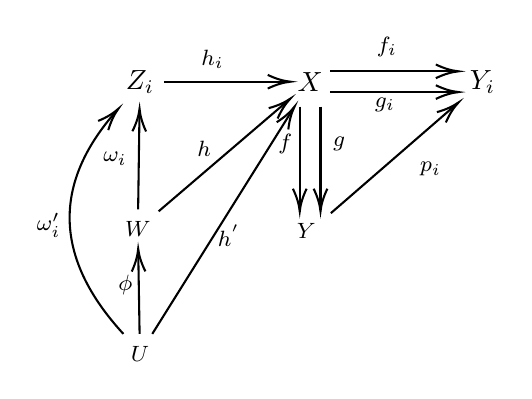
\begin{tikzpicture}[x=0.75pt,y=0.75pt,yscale=-1,xscale=1]
%uncomment if require: \path (0,235); %set diagram left start at 0, and has height of 235


% Text Node
\draw (169,66.14) node    {$Z_{i}$};
% Text Node
\draw (251,66.14) node    {$X$};
% Text Node
\draw (204,55.29) node  [font=\footnotesize]  {$h_{i}$};
% Text Node
\draw (334,66.14) node    {$Y_{i}$};
% Text Node
\draw (288,49.29) node  [font=\footnotesize]  {$f_{i}$};
% Text Node
\draw (287,77.29) node  [font=\footnotesize]  {$g_{i}$};
% Text Node
\draw (251,138.14) node  [font=\footnotesize]  {$Y\ $};
% Text Node
\draw (309,108.29) node  [font=\footnotesize]  {$p_{i}$};
% Text Node
\draw (239,96.29) node  [font=\footnotesize]  {$f$};
% Text Node
\draw (265,96.29) node  [font=\footnotesize]  {$g$};
% Text Node
\draw (168,137.14) node  [font=\footnotesize]  {$W$};
% Text Node
\draw (200,98.29) node  [font=\footnotesize]  {$h$};
% Text Node
\draw (157,103.29) node  [font=\footnotesize]  {$\omega _{i}$};
% Text Node
\draw (169,197.14) node  [font=\footnotesize]  {$U$};
% Text Node
\draw (212,140.29) node  [font=\footnotesize]  {$h^{'}$};
% Text Node
\draw (162,164.29) node  [font=\footnotesize]  {$\phi $};
% Text Node
\draw (125,135.29) node  [font=\footnotesize]  {$\omega _{i} '$};
% Connection
\draw    (180.5,66.14) -- (239.5,66.14) ;
\draw [shift={(241.5,66.14)}, rotate = 180] [color={rgb, 255:red, 0; green, 0; blue, 0 }  ][line width=0.75]    (10.93,-3.29) .. controls (6.95,-1.4) and (3.31,-0.3) .. (0,0) .. controls (3.31,0.3) and (6.95,1.4) .. (10.93,3.29)   ;
% Connection
\draw    (260.5,61.14) -- (320.5,61.14) ;
\draw [shift={(322.5,61.14)}, rotate = 180] [color={rgb, 255:red, 0; green, 0; blue, 0 }  ][line width=0.75]    (10.93,-3.29) .. controls (6.95,-1.4) and (3.31,-0.3) .. (0,0) .. controls (3.31,0.3) and (6.95,1.4) .. (10.93,3.29)   ;
% Connection
\draw    (260.5,71.14) -- (320.5,71.14) ;
\draw [shift={(322.5,71.14)}, rotate = 180] [color={rgb, 255:red, 0; green, 0; blue, 0 }  ][line width=0.75]    (10.93,-3.29) .. controls (6.95,-1.4) and (3.31,-0.3) .. (0,0) .. controls (3.31,0.3) and (6.95,1.4) .. (10.93,3.29)   ;
% Connection
\draw    (261,129.47) -- (320.99,77.43) ;
\draw [shift={(322.5,76.12)}, rotate = 139.06] [color={rgb, 255:red, 0; green, 0; blue, 0 }  ][line width=0.75]    (10.93,-3.29) .. controls (6.95,-1.4) and (3.31,-0.3) .. (0,0) .. controls (3.31,0.3) and (6.95,1.4) .. (10.93,3.29)   ;
% Connection
\draw    (256,78.14) -- (256,126.64) ;
\draw [shift={(256,128.64)}, rotate = 270] [color={rgb, 255:red, 0; green, 0; blue, 0 }  ][line width=0.75]    (10.93,-3.29) .. controls (6.95,-1.4) and (3.31,-0.3) .. (0,0) .. controls (3.31,0.3) and (6.95,1.4) .. (10.93,3.29)   ;
% Connection
\draw    (246,78.14) -- (246,126.64) ;
\draw [shift={(246,128.64)}, rotate = 270] [color={rgb, 255:red, 0; green, 0; blue, 0 }  ][line width=0.75]    (10.93,-3.29) .. controls (6.95,-1.4) and (3.31,-0.3) .. (0,0) .. controls (3.31,0.3) and (6.95,1.4) .. (10.93,3.29)   ;
% Connection
\draw    (178,128.59) -- (239.98,75.57) ;
\draw [shift={(241.5,74.27)}, rotate = 139.46] [color={rgb, 255:red, 0; green, 0; blue, 0 }  ][line width=0.75]    (10.93,-3.29) .. controls (6.95,-1.4) and (3.31,-0.3) .. (0,0) .. controls (3.31,0.3) and (6.95,1.4) .. (10.93,3.29)   ;
% Connection
\draw    (168.13,127.64) -- (168.79,81.14) ;
\draw [shift={(168.82,79.14)}, rotate = 90.81] [color={rgb, 255:red, 0; green, 0; blue, 0 }  ][line width=0.75]    (10.93,-3.29) .. controls (6.95,-1.4) and (3.31,-0.3) .. (0,0) .. controls (3.31,0.3) and (6.95,1.4) .. (10.93,3.29)   ;
% Connection
\draw    (174.95,187.64) -- (242.43,79.84) ;
\draw [shift={(243.49,78.14)}, rotate = 122.04] [color={rgb, 255:red, 0; green, 0; blue, 0 }  ][line width=0.75]    (10.93,-3.29) .. controls (6.95,-1.4) and (3.31,-0.3) .. (0,0) .. controls (3.31,0.3) and (6.95,1.4) .. (10.93,3.29)   ;
% Connection
\draw    (161.03,187.64) .. controls (127.64,151.27) and (126.52,115.45) .. (157.69,80.21) ;
\draw [shift={(158.64,79.14)}, rotate = 132.09] [color={rgb, 255:red, 0; green, 0; blue, 0 }  ][line width=0.75]    (10.93,-3.29) .. controls (6.95,-1.4) and (3.31,-0.3) .. (0,0) .. controls (3.31,0.3) and (6.95,1.4) .. (10.93,3.29)   ;
% Connection
\draw    (168.84,187.64) -- (168.19,148.64) ;
\draw [shift={(168.16,146.64)}, rotate = 89.05] [color={rgb, 255:red, 0; green, 0; blue, 0 }  ][line width=0.75]    (10.93,-3.29) .. controls (6.95,-1.4) and (3.31,-0.3) .. (0,0) .. controls (3.31,0.3) and (6.95,1.4) .. (10.93,3.29)   ;

\end{tikzpicture}

\end{center}
Veamos que $\phi$ es un morfismo conector entre los dos límites.
Sea $i \in I$. Por 
\eqref{eq: fi circ h' igual gi circ h'}, como $(Z_{i}, h_{i})$
es un igualador para $f_{i}$ y $g_{i}$, existe un único morfismo de 
$U$ en $Z_{i}$ que con $h_{i}$ factoriza a $h'$.
Pero
\[
h' = h \circ \phi = (h_{i} \circ \omega_{i}) \circ \phi 
= h_{i} \circ (\omega_{i} \circ \phi),
\]
y también
se tiene \eqref{eq: hi omega i prima = h prima}, luego,
por unicidad concluimos que $\omega_{i}' = \omega_{i} \circ \phi$.

\QEDB
\vspace{0.2cm}

Recordemos estas definiciones;
si $\mathcal{B}$ es una
subcategoría de $\mathcal{A}$, entonces
\begin{itemize}
	\item $\mathcal{B}$ es \textbf{llena} (``full'') si, para cualesquiera
	$X, Y \in Obj(\mathcal{B})$, todo morfismo en 
	$\mathcal{A}$ de $X$ en $Y$ es también un morfismo en 
	$\mathcal{B}$, es decir, si $\mathcal{B}$ contiene a dos objetos
	$X$ y $Y$ de $\mathcal{A}$, entonces contiene a todos los morfismos
	entre ellos.
	\item Si $\mathcal{K}$ es una categoría pequeña y 
	$\mathcal{D}: \mathcal{K} \longrightarrow \mathcal{A}$ es un diagrama,
	se dice que este es \textbf{inicial en $\mathcal{B}$} si
	\[
	(\forall i \in Obj(\mathcal{K}))
	(\exists j \in Obj(\mathcal{K}))
	(\exists a: j \longrightarrow i \in Mor(\mathcal{K})):
	\mathcal{D}(j) \in \mathcal{B}.
	\]
	\item $\mathcal{B}$ es \textbf{fuertemente cerrada en 
	$\mathcal{A}$ bajo $\mathcal{K}-$límites} si 
	para cualquier diagrama 
	$\mathcal{D}: \mathcal{K} \longrightarrow \mathcal{A}$	
	inicial en $\mathcal{B}$ se tiene que el límite 
	$(X, (\alpha_{i})_{i \in Obj(\mathcal{K})})$ para 
	$\mathcal{D}$ cumple que $X \in Obj(\mathcal{B})$.
\end{itemize}

\begin{teo}
(Implicación $6) \Rightarrow 1)$ del Teorema de Caracterización de
Subcategorías Epireflexivas) Sea $\mathcal{A}$ una categoría 
completa, bien potenciada y co-bien potenciada y sea 
$\mathcal{B}$ una sub-categoría de $\mathcal{A}$
llena y cerrada bajo isomorfismos. Si
\begin{itemize}
	\item[$6)$]: $\mathcal{B}$ es fuertemente cerrada en 
	$\mathcal{A}$ bajo productos e igualadores, y
	\item[$1)$]: $\mathcal{B}$ es fuertemente cerrada en $\mathcal{A}$
	bajo $K-$límites para cualquier categoría pequeña $\mathcal{K}$,
\end{itemize}
entonces $6) \Rightarrow 1)$.
\end{teo}
\noindent
\textbf{Demostración.}

Sea $\mathcal{D}: \mathcal{K} \longrightarrow \mathcal{A}$
un diagrama inicial en $\mathcal{B}$; construyamos un límite para 
este y mostremos que el objeto del que parte el límite es 
un objeto de $\mathcal{B}$.

Sea 
\[
S := \{ j \in Obj(\mathcal{K}) | \hspace{0.2cm} 
\mathcal{D}(i) \in Obj(\mathcal{B}) \},
\]
y sea $(X, (p_{i}: X \longrightarrow \mathcal{D}(i))_{i \in S})$
un producto en $\mathcal{A}$ de la familia $(D(i))_{i \in S}$.
\hl{¿A qué se refieren? Sólo sé la definición de producto de monomorfismos
con un mismo codominio, no producto de objetos.}

\begin{center}
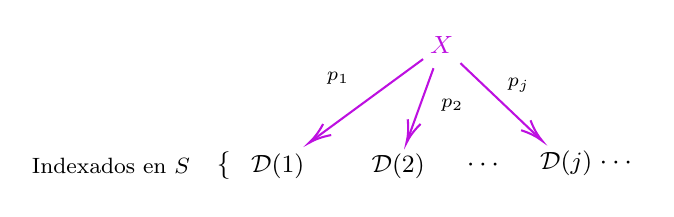
\begin{tikzpicture}[x=0.75pt,y=0.75pt,yscale=-1,xscale=1]
%uncomment if require: \path (0,235); %set diagram left start at 0, and has height of 235


% Text Node
\draw (273,71.14) node  [font=\small,color={rgb, 255:red, 189; green, 16; blue, 224 }  ,opacity=1 ]  {$X$};
% Text Node
\draw (194,129.14) node  [font=\small]  {$\mathcal{D}( 1)$};
% Text Node
\draw (252,129.14) node  [font=\small]  {$\mathcal{D}( 2)$};
% Text Node
\draw (333,128.14) node  [font=\small]  {$\mathcal{D}( j)$};
% Text Node
\draw (294,129.14) node    {$\cdots $};
% Text Node
\draw (223,87.14) node  [font=\scriptsize]  {$p_{1}$};
% Text Node
\draw (278,100.14) node  [font=\scriptsize]  {$p_{2}$};
% Text Node
\draw (310,90.14) node  [font=\scriptsize]  {$p_{j}$};
% Text Node
\draw (358,128.14) node    {$\cdots $};
% Text Node
\draw (74,124) node [anchor=north west][inner sep=0.75pt]  [font=\footnotesize] [align=left] {Indexados en $S$};
% Text Node
\draw (168,129.14) node  [font=\normalsize]  {$\{$};
% Connection
\draw [color={rgb, 255:red, 189; green, 16; blue, 224 }  ,draw opacity=1 ]   (264,77.75) -- (210.59,116.96) ;
\draw [shift={(208.98,118.14)}, rotate = 323.71] [color={rgb, 255:red, 189; green, 16; blue, 224 }  ,draw opacity=1 ][line width=0.75]    (10.93,-3.29) .. controls (6.95,-1.4) and (3.31,-0.3) .. (0,0) .. controls (3.31,0.3) and (6.95,1.4) .. (10.93,3.29)   ;
% Connection
\draw [color={rgb, 255:red, 189; green, 16; blue, 224 }  ,draw opacity=1 ]   (269.02,82.14) -- (256.66,116.26) ;
\draw [shift={(255.98,118.14)}, rotate = 289.9] [color={rgb, 255:red, 189; green, 16; blue, 224 }  ,draw opacity=1 ][line width=0.75]    (10.93,-3.29) .. controls (6.95,-1.4) and (3.31,-0.3) .. (0,0) .. controls (3.31,0.3) and (6.95,1.4) .. (10.93,3.29)   ;
% Connection
\draw [color={rgb, 255:red, 189; green, 16; blue, 224 }  ,draw opacity=1 ]   (282,79.69) -- (319.97,115.77) ;
\draw [shift={(321.42,117.14)}, rotate = 223.53] [color={rgb, 255:red, 189; green, 16; blue, 224 }  ,draw opacity=1 ][line width=0.75]    (10.93,-3.29) .. controls (6.95,-1.4) and (3.31,-0.3) .. (0,0) .. controls (3.31,0.3) and (6.95,1.4) .. (10.93,3.29)   ;

\end{tikzpicture}
\end{center}
Por hipótesis, $X \in Obj(\mathcal{B})$.
Sea la familia
\[
\Lambda = \{ (a, a') \in Mor(\mathcal{K}) \times Mor(\mathcal{K})
  | \hspace{0.2cm} a: j \longrightarrow i, a': j' \longrightarrow i,
  \textit{  con } j, j' \in S \}.
\]
Nótese que, por ser el diagrama $\mathcal{D}$ inicial en 
$\mathcal{B}$, para toda $i \in Obj(\mathcal{K})$ 
existe una pareja $(a, a') \in \Lambda$
de flechas con codominio $i$ (puede ser $a = a'$).
Para cada 
$\lambda = (a: j \longrightarrow i, a': j' \longrightarrow i) \in \Lambda$,
sea $(f_{i}, Y_{i})$ un igualador de los morfismos
$D(a) \circ p_{j}$ y $D(a') \circ p(j')$.

\begin{center}
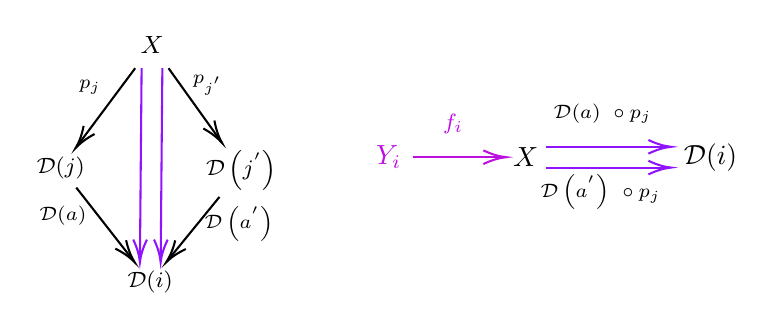
\begin{tikzpicture}[x=0.75pt,y=0.75pt,yscale=-1,xscale=1]
%uncomment if require: \path (0,235); %set diagram left start at 0, and has height of 235
% Text Node
\draw (233,129) node  [color={rgb, 255:red, 189; green, 16; blue, 224 }  ,opacity=1 ]  {$Y_{i}$};
% Text Node
\draw (299,129) node    {$X$};
% Text Node
\draw (388,129) node    {$\mathcal{D}( i)$};
% Text Node
\draw (264,113) node  [font=\footnotesize,color={rgb, 255:red, 189; green, 16; blue, 224 }  ,opacity=1 ]  {$f_{i}$};
% Text Node
\draw (336,108) node  [font=\scriptsize]  {$\mathcal{D}( a) \ \circ p_{j}$};
% Text Node
\draw (335,146) node  [font=\scriptsize]  {$\mathcal{D}\left( a^{'}\right) \ \circ p_{j}$};
% Text Node
\draw (119,75.14) node  [font=\small]  {$X$};
% Text Node
\draw (75,134.14) node  [font=\footnotesize]  {$\mathcal{D}( j)$};
% Text Node
\draw (89,95.14) node  [font=\scriptsize]  {$p_{j}$};
% Text Node
\draw (146,94.14) node  [font=\scriptsize]  {$p_{j^{'}}$};
% Text Node
\draw (162,135.14) node  [font=\footnotesize]  {$\mathcal{D}\left( j^{'}\right)$};
% Text Node
\draw (118,189.14) node  [font=\footnotesize]  {$\mathcal{D}( i)$};
% Text Node
\draw (76,157.14) node  [font=\scriptsize]  {$\mathcal{D}( a)$};
% Text Node
\draw (161,161.14) node  [font=\scriptsize]  {$\mathcal{D}\left( a^{'}\right)$};
% Connection
\draw [color={rgb, 255:red, 189; green, 16; blue, 224 }  ,draw opacity=1 ]   (244.5,129) -- (287.5,129) ;
\draw [shift={(289.5,129)}, rotate = 180] [color={rgb, 255:red, 189; green, 16; blue, 224 }  ,draw opacity=1 ][line width=0.75]    (10.93,-3.29) .. controls (6.95,-1.4) and (3.31,-0.3) .. (0,0) .. controls (3.31,0.3) and (6.95,1.4) .. (10.93,3.29)   ;
% Connection
\draw [color={rgb, 255:red, 144; green, 19; blue, 254 }  ,draw opacity=1 ]   (308.5,124) -- (367,124) ;
\draw [shift={(369,124)}, rotate = 180] [color={rgb, 255:red, 144; green, 19; blue, 254 }  ,draw opacity=1 ][line width=0.75]    (10.93,-3.29) .. controls (6.95,-1.4) and (3.31,-0.3) .. (0,0) .. controls (3.31,0.3) and (6.95,1.4) .. (10.93,3.29)   ;
% Connection
\draw [color={rgb, 255:red, 144; green, 19; blue, 254 }  ,draw opacity=1 ]   (308.5,134) -- (367,134) ;
\draw [shift={(369,134)}, rotate = 180] [color={rgb, 255:red, 144; green, 19; blue, 254 }  ,draw opacity=1 ][line width=0.75]    (10.93,-3.29) .. controls (6.95,-1.4) and (3.31,-0.3) .. (0,0) .. controls (3.31,0.3) and (6.95,1.4) .. (10.93,3.29)   ;
% Connection
\draw    (110.8,86.14) -- (83.28,123.04) ;
\draw [shift={(82.08,124.64)}, rotate = 306.71] [color={rgb, 255:red, 0; green, 0; blue, 0 }  ][line width=0.75]    (10.93,-3.29) .. controls (6.95,-1.4) and (3.31,-0.3) .. (0,0) .. controls (3.31,0.3) and (6.95,1.4) .. (10.93,3.29)   ;
% Connection
\draw    (126.88,86.14) -- (151.52,120.52) ;
\draw [shift={(152.68,122.14)}, rotate = 234.37] [color={rgb, 255:red, 0; green, 0; blue, 0 }  ][line width=0.75]    (10.93,-3.29) .. controls (6.95,-1.4) and (3.31,-0.3) .. (0,0) .. controls (3.31,0.3) and (6.95,1.4) .. (10.93,3.29)   ;
% Connection
\draw    (151.41,148.14) -- (127,178.09) ;
\draw [shift={(125.74,179.64)}, rotate = 309.17] [color={rgb, 255:red, 0; green, 0; blue, 0 }  ][line width=0.75]    (10.93,-3.29) .. controls (6.95,-1.4) and (3.31,-0.3) .. (0,0) .. controls (3.31,0.3) and (6.95,1.4) .. (10.93,3.29)   ;
% Connection
\draw    (82.43,143.64) -- (109.34,178.07) ;
\draw [shift={(110.57,179.64)}, rotate = 231.98] [color={rgb, 255:red, 0; green, 0; blue, 0 }  ][line width=0.75]    (10.93,-3.29) .. controls (6.95,-1.4) and (3.31,-0.3) .. (0,0) .. controls (3.31,0.3) and (6.95,1.4) .. (10.93,3.29)   ;
% Connection
\draw [color={rgb, 255:red, 144; green, 19; blue, 254 }  ,draw opacity=1 ]   (123.9,86.14) -- (123.1,177.64) ;
\draw [shift={(123.08,179.64)}, rotate = 270.5] [color={rgb, 255:red, 144; green, 19; blue, 254 }  ,draw opacity=1 ][line width=0.75]    (10.93,-3.29) .. controls (6.95,-1.4) and (3.31,-0.3) .. (0,0) .. controls (3.31,0.3) and (6.95,1.4) .. (10.93,3.29)   ;
% Connection
\draw [color={rgb, 255:red, 144; green, 19; blue, 254 }  ,draw opacity=1 ]   (113.9,86.14) -- (113.1,177.64) ;
\draw [shift={(113.08,179.64)}, rotate = 270.5] [color={rgb, 255:red, 144; green, 19; blue, 254 }  ,draw opacity=1 ][line width=0.75]    (10.93,-3.29) .. controls (6.95,-1.4) and (3.31,-0.3) .. (0,0) .. controls (3.31,0.3) and (6.95,1.4) .. (10.93,3.29)   ;

\end{tikzpicture}
\end{center}
\noindent
Entonces, como $X \in Obj(\mathcal{B})$, por hipótesis se sigue que
\begin{equation}
	\label{eq: todos los Yi en obj B}
	\forall i : Y_{i} \in Obj(\mathcal{B}).
\end{equation}
Sea ahora $(Z, ((g_{\lambda})_{\lambda \in \Lambda}, f))$
una intersección de los monomorfismos $f_{i}$. 
\begin{center}
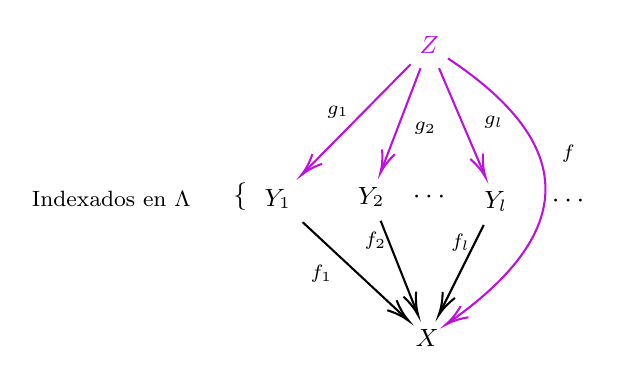
\begin{tikzpicture}[x=0.75pt,y=0.75pt,yscale=-1,xscale=1]
%uncomment if require: \path (0,235); %set diagram left start at 0, and has height of 235


% Text Node
\draw (267,55.14) node  [font=\small,color={rgb, 255:red, 189; green, 16; blue, 224 }  ,opacity=1 ]  {$Z$};
% Text Node
\draw (194,129.14) node  [font=\small]  {$Y_{1}$};
% Text Node
\draw (239,128.14) node  [font=\small]  {$Y_{2}$};
% Text Node
\draw (299,130.14) node  [font=\small]  {$Y_{l}$};
% Text Node
\draw (268,128.14) node    {$\cdots $};
% Text Node
\draw (223,87.14) node  [font=\scriptsize]  {$g_{1}$};
% Text Node
\draw (265,95.14) node  [font=\scriptsize]  {$g_{2}$};
% Text Node
\draw (298,92.14) node  [font=\scriptsize]  {$g_{l}$};
% Text Node
\draw (335,130.14) node    {$\cdots $};
% Text Node
\draw (74,124) node [anchor=north west][inner sep=0.75pt]  [font=\footnotesize] [align=left] {Indexados en $\Lambda$};
% Text Node
\draw (176,128.14) node  [font=\normalsize]  {$\{$};
% Text Node
\draw (266,196.14) node  [font=\small,color={rgb, 255:red, 0; green, 0; blue, 0 }  ,opacity=1 ]  {$X$};
% Text Node
\draw (215,165.14) node  [font=\scriptsize]  {$f_{1}$};
% Text Node
\draw (241,149.14) node  [font=\scriptsize]  {$f_{2}$};
% Text Node
\draw (282,150.14) node  [font=\scriptsize]  {$f_{l}$};
% Text Node
\draw (334,107.14) node  [font=\scriptsize]  {$f$};
% Connection
\draw [color={rgb, 255:red, 189; green, 16; blue, 224 }  ,draw opacity=1 ]   (258,64.27) -- (206.75,116.22) ;
\draw [shift={(205.34,117.64)}, rotate = 314.61] [color={rgb, 255:red, 189; green, 16; blue, 224 }  ,draw opacity=1 ][line width=0.75]    (10.93,-3.29) .. controls (6.95,-1.4) and (3.31,-0.3) .. (0,0) .. controls (3.31,0.3) and (6.95,1.4) .. (10.93,3.29)   ;
% Connection
\draw [color={rgb, 255:red, 189; green, 16; blue, 224 }  ,draw opacity=1 ]   (262.78,66.14) -- (244.13,114.78) ;
\draw [shift={(243.41,116.64)}, rotate = 290.98] [color={rgb, 255:red, 189; green, 16; blue, 224 }  ,draw opacity=1 ][line width=0.75]    (10.93,-3.29) .. controls (6.95,-1.4) and (3.31,-0.3) .. (0,0) .. controls (3.31,0.3) and (6.95,1.4) .. (10.93,3.29)   ;
% Connection
\draw [color={rgb, 255:red, 189; green, 16; blue, 224 }  ,draw opacity=1 ]   (271.69,66.14) -- (293.31,116.8) ;
\draw [shift={(294.09,118.64)}, rotate = 246.89] [color={rgb, 255:red, 189; green, 16; blue, 224 }  ,draw opacity=1 ][line width=0.75]    (10.93,-3.29) .. controls (6.95,-1.4) and (3.31,-0.3) .. (0,0) .. controls (3.31,0.3) and (6.95,1.4) .. (10.93,3.29)   ;
% Connection
\draw    (206,140.31) -- (255.54,186.41) ;
\draw [shift={(257,187.77)}, rotate = 222.94] [color={rgb, 255:red, 0; green, 0; blue, 0 }  ][line width=0.75]    (10.93,-3.29) .. controls (6.95,-1.4) and (3.31,-0.3) .. (0,0) .. controls (3.31,0.3) and (6.95,1.4) .. (10.93,3.29)   ;
% Connection
\draw    (243.57,139.64) -- (260.89,183.28) ;
\draw [shift={(261.63,185.14)}, rotate = 248.34] [color={rgb, 255:red, 0; green, 0; blue, 0 }  ][line width=0.75]    (10.93,-3.29) .. controls (6.95,-1.4) and (3.31,-0.3) .. (0,0) .. controls (3.31,0.3) and (6.95,1.4) .. (10.93,3.29)   ;
% Connection
\draw    (293.25,141.64) -- (272.39,183.35) ;
\draw [shift={(271.5,185.14)}, rotate = 296.57] [color={rgb, 255:red, 0; green, 0; blue, 0 }  ][line width=0.75]    (10.93,-3.29) .. controls (6.95,-1.4) and (3.31,-0.3) .. (0,0) .. controls (3.31,0.3) and (6.95,1.4) .. (10.93,3.29)   ;
% Connection
\draw [color={rgb, 255:red, 189; green, 16; blue, 224 }  ,draw opacity=1 ]   (276,61.42) .. controls (338.64,102.84) and (338.62,145.35) .. (275.95,188.97) ;
\draw [shift={(275,189.63)}, rotate = 325.43] [color={rgb, 255:red, 189; green, 16; blue, 224 }  ,draw opacity=1 ][line width=0.75]    (10.93,-3.29) .. controls (6.95,-1.4) and (3.31,-0.3) .. (0,0) .. controls (3.31,0.3) and (6.95,1.4) .. (10.93,3.29)   ;

\end{tikzpicture}
\end{center}
Según el Lema 7.10, 
\eqref{eq: todos los Yi en obj B} implica que
\[
Z \in Obj(\mathcal{B}).
\]
Para todo $i \in Obj(\mathcal{K})$, vamos a constuir un morfismo
$\alpha_{i}: Z \longrightarrow \mathcal{D}(i)$ como sigue:
\begin{itemize}
	\item Si $i \in S$, entonces
	\begin{equation}
		\label{eq: defi de alpha i si i en S}
		\alpha_{i}:= p_{i} \circ f : Z \longrightarrow \mathcal{D}(i). 
	\end{equation}
	\item Si $i \not\in S$, es decir, 
	si $\mathcal{D}(i) \not\in Obj(\mathbb{B})$, por hipótesis existen
	un $\mathcal{K}-$objeto $j \in S$ y un $\mathcal{K}$ morfismo 
	$a: j \longrightarrow i$. Defínase entonces
	\begin{equation}
		\label{eq: defi de alpha i si i no esta en S}
		\alpha_{i}:= \mathcal{D}(a) \circ
		p_{j} \circ f : Z \longrightarrow \mathcal{D}(i). 
	\end{equation}
\end{itemize}
\begin{center}
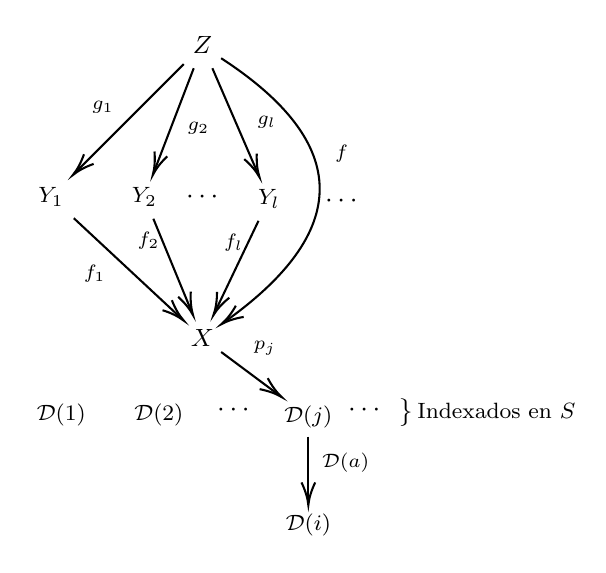
\begin{tikzpicture}[x=0.75pt,y=0.75pt,yscale=-1,xscale=1]
%uncomment if require: \path (0,300); %set diagram left start at 0, and has height of 300


% Text Node
\draw (135,16.14) node  [font=\small,color={rgb, 255:red, 0; green, 0; blue, 0 }  ,opacity=1 ]  {$Z$};
% Text Node
\draw (62,89.14) node  [font=\footnotesize]  {$Y_{1}$};
% Text Node
\draw (107,89.14) node  [font=\footnotesize]  {$Y_{2}$};
% Text Node
\draw (167,90.14) node  [font=\footnotesize]  {$Y_{l}$};
% Text Node
\draw (136,89.14) node    {$\cdots $};
% Text Node
\draw (87,46.14) node  [font=\scriptsize]  {$g_{1}$};
% Text Node
\draw (133,56.14) node  [font=\scriptsize]  {$g_{2}$};
% Text Node
\draw (166,53.14) node  [font=\scriptsize]  {$g_{l}$};
% Text Node
\draw (203,91.14) node    {$\cdots $};
% Text Node
\draw (135,157.14) node  [font=\small,color={rgb, 255:red, 0; green, 0; blue, 0 }  ,opacity=1 ]  {$X$};
% Text Node
\draw (83,126.14) node  [font=\scriptsize]  {$f_{1}$};
% Text Node
\draw (109,110.14) node  [font=\scriptsize]  {$f_{2}$};
% Text Node
\draw (150,111.14) node  [font=\scriptsize]  {$f_{l}$};
% Text Node
\draw (202,68.14) node  [font=\scriptsize]  {$f$};
% Text Node
\draw (67,194.14) node  [font=\footnotesize]  {$\mathcal{D}( 1)$};
% Text Node
\draw (151,192.14) node    {$\cdots $};
% Text Node
\draw (114,194.14) node  [font=\footnotesize]  {$\mathcal{D}( 2)$};
% Text Node
\draw (186,195.14) node  [font=\footnotesize]  {$\mathcal{D}( j)$};
% Text Node
\draw (214,192.14) node    {$\cdots $};
% Text Node
\draw (186,247.14) node  [font=\footnotesize]  {$\mathcal{D}( i)$};
% Text Node
\draw (204,217.14) node  [font=\scriptsize]  {$\mathcal{D}( a)$};
% Text Node
\draw (165,162.14) node  [font=\scriptsize]  {$p_{j}$};
% Text Node
\draw (233,193.14) node  [font=\normalsize]  {$\}$};
% Text Node
\draw (237,187) node [anchor=north west][inner sep=0.75pt]  [font=\footnotesize] [align=left] {Indexados en $S$};
% Connection
\draw [color={rgb, 255:red, 0; green, 0; blue, 0 }  ,draw opacity=1 ]   (126,25.14) -- (73.91,77.23) ;
\draw [shift={(72.5,78.64)}, rotate = 315] [color={rgb, 255:red, 0; green, 0; blue, 0 }  ,draw opacity=1 ][line width=0.75]    (10.93,-3.29) .. controls (6.95,-1.4) and (3.31,-0.3) .. (0,0) .. controls (3.31,0.3) and (6.95,1.4) .. (10.93,3.29)   ;
% Connection
\draw [color={rgb, 255:red, 0; green, 0; blue, 0 }  ,draw opacity=1 ]   (130.78,27.14) -- (111.74,76.78) ;
\draw [shift={(111.03,78.64)}, rotate = 290.98] [color={rgb, 255:red, 0; green, 0; blue, 0 }  ,draw opacity=1 ][line width=0.75]    (10.93,-3.29) .. controls (6.95,-1.4) and (3.31,-0.3) .. (0,0) .. controls (3.31,0.3) and (6.95,1.4) .. (10.93,3.29)   ;
% Connection
\draw [color={rgb, 255:red, 0; green, 0; blue, 0 }  ,draw opacity=1 ]   (139.76,27.14) -- (161.67,77.81) ;
\draw [shift={(162.46,79.64)}, rotate = 246.61] [color={rgb, 255:red, 0; green, 0; blue, 0 }  ,draw opacity=1 ][line width=0.75]    (10.93,-3.29) .. controls (6.95,-1.4) and (3.31,-0.3) .. (0,0) .. controls (3.31,0.3) and (6.95,1.4) .. (10.93,3.29)   ;
% Connection
\draw [color={rgb, 255:red, 0; green, 0; blue, 0 }  ,draw opacity=1 ]   (73,99.39) -- (124.54,147.4) ;
\draw [shift={(126,148.76)}, rotate = 222.97] [color={rgb, 255:red, 0; green, 0; blue, 0 }  ,draw opacity=1 ][line width=0.75]    (10.93,-3.29) .. controls (6.95,-1.4) and (3.31,-0.3) .. (0,0) .. controls (3.31,0.3) and (6.95,1.4) .. (10.93,3.29)   ;
% Connection
\draw [color={rgb, 255:red, 0; green, 0; blue, 0 }  ,draw opacity=1 ]   (111.32,99.64) -- (129.71,144.29) ;
\draw [shift={(130.47,146.14)}, rotate = 247.62] [color={rgb, 255:red, 0; green, 0; blue, 0 }  ,draw opacity=1 ][line width=0.75]    (10.93,-3.29) .. controls (6.95,-1.4) and (3.31,-0.3) .. (0,0) .. controls (3.31,0.3) and (6.95,1.4) .. (10.93,3.29)   ;
% Connection
\draw [color={rgb, 255:red, 0; green, 0; blue, 0 }  ,draw opacity=1 ]   (161.99,100.64) -- (141.12,144.34) ;
\draw [shift={(140.25,146.14)}, rotate = 295.53] [color={rgb, 255:red, 0; green, 0; blue, 0 }  ,draw opacity=1 ][line width=0.75]    (10.93,-3.29) .. controls (6.95,-1.4) and (3.31,-0.3) .. (0,0) .. controls (3.31,0.3) and (6.95,1.4) .. (10.93,3.29)   ;
% Connection
\draw [color={rgb, 255:red, 0; green, 0; blue, 0 }  ,draw opacity=1 ]   (144,22.32) .. controls (206.96,63.31) and (207.28,105.83) .. (144.94,149.86) ;
\draw [shift={(144,150.53)}, rotate = 325.02] [color={rgb, 255:red, 0; green, 0; blue, 0 }  ,draw opacity=1 ][line width=0.75]    (10.93,-3.29) .. controls (6.95,-1.4) and (3.31,-0.3) .. (0,0) .. controls (3.31,0.3) and (6.95,1.4) .. (10.93,3.29)   ;
% Connection
\draw    (186,204.64) -- (186,235.64) ;
\draw [shift={(186,237.64)}, rotate = 270] [color={rgb, 255:red, 0; green, 0; blue, 0 }  ][line width=0.75]    (10.93,-3.29) .. controls (6.95,-1.4) and (3.31,-0.3) .. (0,0) .. controls (3.31,0.3) and (6.95,1.4) .. (10.93,3.29)   ;
% Connection
\draw    (144,163.85) -- (171.65,184.45) ;
\draw [shift={(173.25,185.64)}, rotate = 216.69] [color={rgb, 255:red, 0; green, 0; blue, 0 }  ][line width=0.75]    (10.93,-3.29) .. controls (6.95,-1.4) and (3.31,-0.3) .. (0,0) .. controls (3.31,0.3) and (6.95,1.4) .. (10.93,3.29)   ;

\end{tikzpicture}
\end{center}
Mostremos que la definición 
\eqref{eq: defi de alpha i si i no esta en S} de 
$\alpha_{i}$ cuando $i \not\in S$ no depende de la elección de 
$j$, es decir, que si existe otro $j' \in S$ y otro morfismo
$a': j' \longrightarrow i$, entonces
\[
\mathcal{D}(a) \circ p_{j} \circ f = \mathcal{D}(a') \circ p_{j'} 
\circ f.
\]

\begin{center}
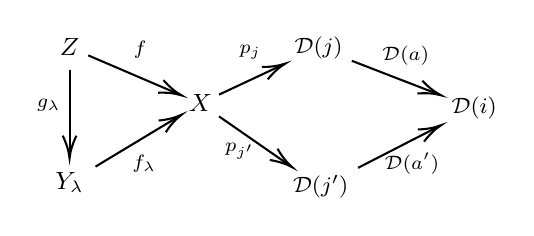
\begin{tikzpicture}[x=0.75pt,y=0.75pt,yscale=-1,xscale=1]
%uncomment if require: \path (0,235); %set diagram left start at 0, and has height of 235


% Text Node
\draw (81,55) node  [font=\small,color={rgb, 255:red, 0; green, 0; blue, 0 }  ,opacity=1 ]  {$Z$};
% Text Node
\draw (81,120) node  [font=\small,color={rgb, 255:red, 0; green, 0; blue, 0 }  ,opacity=1 ]  {$Y_{\lambda }$};
% Text Node
\draw (144,82) node  [font=\small,color={rgb, 255:red, 0; green, 0; blue, 0 }  ,opacity=1 ]  {$X$};
% Text Node
\draw (201,55.29) node  [font=\footnotesize]  {$\mathcal{D}( j)$};
% Text Node
\draw (202,122.29) node  [font=\footnotesize]  {$\mathcal{D}( j')$};
% Text Node
\draw (276,84.29) node  [font=\footnotesize]  {$\mathcal{D}( i)$};
% Text Node
\draw (168,57.14) node  [font=\scriptsize]  {$p_{j}$};
% Text Node
\draw (163,105.14) node  [font=\scriptsize]  {$p_{j'}$};
% Text Node
\draw (243,59) node  [font=\scriptsize]  {$\mathcal{D}( a)$};
% Text Node
\draw (246,111) node  [font=\scriptsize]  {$\mathcal{D}( a')$};
% Text Node
\draw (115,56) node  [font=\scriptsize]  {$f$};
% Text Node
\draw (117,111) node  [font=\scriptsize]  {$f_{\lambda }$};
% Text Node
\draw (71,83) node  [font=\scriptsize]  {$g_{\lambda }$};
% Connection
\draw    (90,58.86) -- (133.16,77.36) ;
\draw [shift={(135,78.14)}, rotate = 203.2] [color={rgb, 255:red, 0; green, 0; blue, 0 }  ][line width=0.75]    (10.93,-3.29) .. controls (6.95,-1.4) and (3.31,-0.3) .. (0,0) .. controls (3.31,0.3) and (6.95,1.4) .. (10.93,3.29)   ;
% Connection
\draw    (93.5,112.46) -- (133.29,88.46) ;
\draw [shift={(135,87.43)}, rotate = 148.9] [color={rgb, 255:red, 0; green, 0; blue, 0 }  ][line width=0.75]    (10.93,-3.29) .. controls (6.95,-1.4) and (3.31,-0.3) .. (0,0) .. controls (3.31,0.3) and (6.95,1.4) .. (10.93,3.29)   ;
% Connection
\draw    (81,66) -- (81,106.5) ;
\draw [shift={(81,108.5)}, rotate = 270] [color={rgb, 255:red, 0; green, 0; blue, 0 }  ][line width=0.75]    (10.93,-3.29) .. controls (6.95,-1.4) and (3.31,-0.3) .. (0,0) .. controls (3.31,0.3) and (6.95,1.4) .. (10.93,3.29)   ;
% Connection
\draw    (153,77.78) -- (183.19,63.63) ;
\draw [shift={(185,62.78)}, rotate = 154.89] [color={rgb, 255:red, 0; green, 0; blue, 0 }  ][line width=0.75]    (10.93,-3.29) .. controls (6.95,-1.4) and (3.31,-0.3) .. (0,0) .. controls (3.31,0.3) and (6.95,1.4) .. (10.93,3.29)   ;
% Connection
\draw    (153,88.25) -- (186.68,111.64) ;
\draw [shift={(188.32,112.79)}, rotate = 214.78] [color={rgb, 255:red, 0; green, 0; blue, 0 }  ][line width=0.75]    (10.93,-3.29) .. controls (6.95,-1.4) and (3.31,-0.3) .. (0,0) .. controls (3.31,0.3) and (6.95,1.4) .. (10.93,3.29)   ;
% Connection
\draw    (217,61.47) -- (258.13,77.38) ;
\draw [shift={(260,78.1)}, rotate = 201.14] [color={rgb, 255:red, 0; green, 0; blue, 0 }  ][line width=0.75]    (10.93,-3.29) .. controls (6.95,-1.4) and (3.31,-0.3) .. (0,0) .. controls (3.31,0.3) and (6.95,1.4) .. (10.93,3.29)   ;
% Connection
\draw    (220,113.04) -- (258.22,93.42) ;
\draw [shift={(260,92.5)}, rotate = 152.82] [color={rgb, 255:red, 0; green, 0; blue, 0 }  ][line width=0.75]    (10.93,-3.29) .. controls (6.95,-1.4) and (3.31,-0.3) .. (0,0) .. controls (3.31,0.3) and (6.95,1.4) .. (10.93,3.29)   ;

\end{tikzpicture}
\end{center}
\hl{¿Cómo? Supongo que tengo que usar que, para toda $\lambda \in \Lambda$,
$(f_{\lambda}, Y)$ es igualador de las composiciones marcadas.}

Si mostramos que $(Z, (\alpha_{i})_{i \in Obj(\mathcal{K})})$
es un límite para el diagrama 
$\mathcal{D}: \mathcal{K} \longrightarrow \mathcal{A}$, puesto que 
ya expusimos a $Z$ como un objeto de $\mathcal{B}$, habremos terminado.
\hl{Me falta esto...}
\QEDB
\vspace{0.2cm}









\end{document}